\documentclass[11pt,letterpaper]{article}
\usepackage[utf8]{inputenc}
\usepackage[spanish,USenglish]{babel}
\usepackage{amsmath}
\usepackage{amsfonts}
\usepackage{amssymb}
\usepackage{amsthm}
\usepackage{graphicx}
\usepackage[left=2cm,right=2cm,top=2cm,bottom=2cm]{geometry}
\usepackage{flushend}
\usepackage{pgf,tikz, pgfplots}
\usetikzlibrary{arrows}
\pgfplotsset{compat=1.15}
\usepackage{pgf,tikz,pgfplots}
%escribir programas
\usepackage{listings}
\usepackage{algpseudocode}
\usepackage{algorithm}
\renewcommand{\algorithmicrequire}{\textbf{Input:}}
\renewcommand{\algorithmicensure}{\textbf{Output:}}

%encabezado
\usepackage{fancyhdr}
\pagestyle{fancy}
\fancyhf{}
\fancyhead[RO]{\thepage} % Números de página en las esquinas de los encabezados
%%%%%%%%%%%%%%%%%%%% BOXES %%%%%%%%%%%%%%%%%%%
\usepackage{bm}
\newcommand{\commentedbox}[2]{%
	\mbox{
		\begin{tabular}[t]{@{}c@{}}
			$\boxed{\displaystyle#1}$\\
			#2
		\end{tabular}%
	}%
}
\usepackage{framed}
\usepackage{wrapfig}\definecolor{shadecolor}{RGB}{224,238,238}
%%%%%%%%%%%%%%%%%%%%%%%%% DEFINITIONS %%%%%%%%%%%%%%%%%%%%%%%%
\theoremstyle{definition}
\newtheorem{defi}{Definición}[section]%Para definiciones
\theoremstyle{definition}
\newtheorem{teo}{Teorema}[section]%Para definiciones
\newtheorem{prop}{Proposición}
\theoremstyle{definition}
\newtheorem{ej}{Ejemplo}[section]
\newtheorem{lem}{Lema}
\newtheorem{prblm}{Problema}
\newtheorem{col}{Corolario}[section]



\title{\textbf{Tarea 12: Método BFGS y Descenso Gradiente}\\ Optimización I \\ \Large {Maestría en Computación}\\ \Large {Centro de Investigación en Matemáticas}}
\author{Esteban Reyes Saldaña \\ esteban.reyes@cimat.mx}

\begin{document}

\selectlanguage{spanish}
\twocolumn[
\begin{@twocolumnfalse}
	\maketitle
	\begin{center}\rule{0.9\textwidth}{0.1mm} \end{center}
	\begin{abstract}
		\normalsize{En esta tarea se utilizó el método de descenso gradiente con paso exacto y el método BFGS para minimizar una función de clasificación binaria sobre el conjunto de datos  \textit{mnist.pkl.gz}. En este caso el conjunto de datos corresponde a imágenes de números dígitos escritos a mano. Se presenta a continuación una descripción general de dicha función  así como el pseudocódigo de los métodos implementados. Debido a la complejidad analítica de la función, se utilizó una aproximación del gradiente y del Hessiano. En los resultados se incluyen pruebas de descenso gradiente y del método BFGS .Finalmente se incluyen conclusiones observadas a partir de la experimentación.}
	\begin{center}\rule{0.9\textwidth}{0.1mm} \end{center}
	\end{abstract}
\end{@twocolumnfalse}]

\section{Introducción}
\subsection{Descenso Gradiente}
Algunos resultados relevantes sobre el gradiente, vistos en la tarea pasada son
\begin{shaded*}
\begin{teo}
	Sea $ f: \mathbb{R}^n \to \mathbb{R} $ una función continuamente diferenciable. Entonces para toda $ x  \in dom(f) $, $ \nabla f(x) $ es perpendicular al conjunto de nivel
	\[ S = \{ x \in \mathbb{R}^n | f(x) = c, c\textup{ constante.} \} \]
\end{teo}
\end{shaded*}

\begin{shaded*}
\begin{teo}\label{max_}
	Sea $ f: \mathbb{R}^n \to \mathbb{R} $ una función continuamente diferenciable. Entonces la dirección donde $ f(x) $ crece más rápido es $ \nabla f(x) $.
\end{teo}
\end{shaded*}

\begin{col}
	Bajo las condiciones del Teorema (\ref{max_}), $ f(x) $ decrece más rápido en la dirección $ - \nabla f(x) $.
\end{col}

\begin{shaded*}
\begin{defi}
	Una \textbf{dirección de descenso} $ d \in \mathbb{R}^n $ para $ f \in \mathcal{C}^1 $ es un vector tal que
	\[ f(x + t d) < f(x) \]
	para $ t \in (0, T) $. Es decir, permite que el punto $ x $ más cerca al mínimo local $ x^* $ de la función objetivo $ f: \mathbb{R}^n \to \mathbb{R} $.
\end{defi}
\end{shaded*}

\begin{shaded*}
\begin{teo}
	Si $ g(x)^T d < 0 $ entonces $ d $ es una dirección de descenso.
\end{teo}
\end{shaded*}
\textbf{Observación.} La dirección 
\[ d_k = - g(x_k) \]
es la elección más obvia de una dirección de búsqueda.

\subsection{Método BFGS}
El método de Newton es una algoritmo iterativo que permite obtener el óptimo $ x^* $ de una función $ 2 $ veces continuamente diferenciable $ f : \mathbb{R}^n \to \mathbb{R} $. Dicho algoritmo es optimización sin restricciones. 
\\
A partir de un punto inicial $ x_0 $ se genera una secuencia $ \{x_k\} $,
\begin{shaded*}
	\begin{equation*}
		x_{k+1} = x_k - ( \nabla^2 f_k)^{-1} \nabla f_k
	\end{equation*}
\end{shaded*}
donde $  \nabla^2 f_k = \nabla^2 f(x_k) $ es el Hessiano y $ \nabla f_k = \nabla f(x_k) $ es el gradiente.
\\
Para encontrar el nuevo punto $ x_{k+1} $ a partir de $ x_k $ se define $ d = x - x_k $ y se usa la aproximación de Taylor de segundo orden de la función
\begin{shaded*}
	\begin{equation*}
		m_k (d) = f_k + f_k d + \dfrac{1}{2} d^T \nabla^2 f_k d
	\end{equation*}
\end{shaded*}
donde el tamaño de paso se obtiene calculando el gradiente, igualidando a cero y resolviendo para $ p $.
\\
Una de la \textbf{problemáticas} del método de Newton es que requiere calcular el Hessiano $ \nabla^2 f_k $ cual pueder ser muy costoso. Más aún, requiere el cálculo de la inversa del Hessiano,
\[ d_k = - (\nabla^2 f_k)^{-1} \nabla f_k. \]
Otro problema es que no se puede garantizar que $ d_k $ sea una dirección de descenso, i.e, puede suceder que
\[ d_k^T \nabla f_k = - \nabla^T f_k (\nabla^2 f_k)^{-1} \nabla f_k > 0 \]
en alguna o varias iteraciones.
\\
Una alternativa de solución, cuando $ d_k $ no es una dirección de descenso, es modificar el Hessiano añadiendo una matrix $ E_k $ de modo que la nueva matrix $ B_k = \nabla^2 f_k + E_k $ sea definida positiva.
\\
La alternativa anterior garantiza que la dirección $ d_k $ sea de descenso, sin embargo, requiere del cálculo de Hessiano. Además necesita de un algoritmo que garantice que la nueva matriz $ B_k $ sea definida positiva (p.e. Cholesky).
\\
\textbf{¿Existe alguna otra alternativa?}
\begin{itemize}
	\item Los métodos cuasi-newton construyen un modelo que se
	basa en medir los cambios del gradiente.
	\item Solo requieren del cálculo del gradiente, similar al
	algoritmo de máximo descenso.
	\item Su comportamiento es superior al algoritmo de máximo
	descenso.
	\item En lugar de calcular el Hessiano en cada iteración se
	propone un método que permite calcular una secuencia $ B_k $ usando la curvatura medida en el paso actual.
\end{itemize}
 
\subsection{Datos MNIST}
Los datos utilizados corresponden a la base de datos MNIST. Que son imágenes de números dígitos escritos a mano. Las imágenes tiene  dimensión $ 28 \times 28 $ y la distribución de los datos está dada por
\begin{center}
	\begin{tabular}{|c|c|}
	\hline
	Datos & Cantidad \\
	\hline
	Entrenamiento & 50000 \\
	\hline
	Pruebas & 10000 \\
	\hline
	Validación & 10000 \\
	\hline
\end{tabular}
\end{center}
A continuación se muestra un ejemplo del conjunto de entrenamiento
\begin{center}
	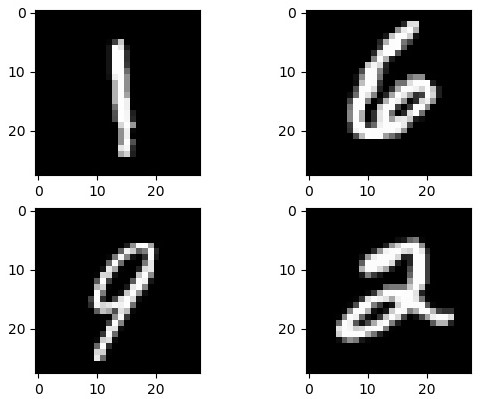
\includegraphics[width=0.8\linewidth]{graficas/example}
\end{center}
Dado que la función $ F_\theta (\theta) $ corresponde a clasificación binaria, la experimentaición se realizó con las imágenes de etiqueta cero y uno.

\section{Método}
\subsection{Aproximación del Gradiente}
Algunas veces puede resultar difícil calcular el gradiente de una función de manera analítica dada su complejidad en cuanto a variables. En vez de hacer eso se puede usar una aproximación de primer orden. Usando expansión de Taylor de primer orden sobre una función $ f(x) $ tenemos que
\begin{shaded*}
	\begin{equation}
		f(x + hd) = f(x) + h \nabla^T f(x) d + O (h^2)
	\end{equation}
\end{shaded*}
donde $ d $ es un vector unitario, es decir, $ || d || = 1 $. Por notivos de notación, llamaremos $ \nabla f(x) = g $ y $ \nabla^2 f(x) = H $. Así que 
\begin{shaded*}
	\begin{equation*}
		f(x + hd) = f(x) + h g^T d + O (h^2)
	\end{equation*}
\end{shaded*}

Si $ d = e_i $, donde $ e_i $ denota al vector canónico $ i $, i.e.,
\begin{equation*}
	e_i^T = \left[ 0, 0, \dots, \underbrace{1}_{i}, \dots, 0 \right], i = 1, \dots, n.
\end{equation*}
Las componentes no nulas correspondientes al $ i $-ésimo componente de $ e_i $ quedan como
\begin{eqnarray*}
	f(x + h e_i) & = & f(x) + h g^T e_i + O(h^2) \\
	& = & f(x) + h g_i + O(h^2).
\end{eqnarray*}
reordenando términos tenemos
\begin{shaded*}
	\begin{equation*}
		g_i \approx \dfrac{f(x + h e_i) - f(x)}{h}
	\end{equation*}
\end{shaded*}
Así obtenemos una \textbf{aproxiamción de primer orden} para $ g $. De manera similar podemos aproximar el Hessiano. Sin embargo, para descneso gradiente con paso exacto, estamos interesados en encontrar $ Hd $, esto se puede aproximar mediante
\begin{equation*}
	g(x + hd) = g + h H d + O (h^2),
\end{equation*}
reordenando términos obtenemos
\begin{shaded*}
	\begin{equation*}
		Hd \approx \dfrac{g(x + hd) - g}{h}
	\end{equation*}
\end{shaded*}
\subsection{Método BFGS}
En el BFGS la idea es calcular la aproximacion de matriz inversa del Hessiano $ H_{k+1} $ basado en $ B_{k+1} $.
Para ello se considera la ecuación $ DFP $ con $ \rho_k = \dfrac{1}{s_k y_k} $
y se usa
\begin{shaded*}
	\begin{equation*}
		B_{k+1} = (I - \rho_k y_k s_k^T) B_k ( I - \rho_k s_k y_k^T) + \rho_k y_k y_k^T
	\end{equation*}
\end{shaded*}
y las relaciones
\begin{shaded*}
	\begin{eqnarray*}
		B_{k+1} s_k & = & y_k \\
		H_{k+1} y_k & = & s_k.
	\end{eqnarray*}
\end{shaded*}
Ahora, $ \rho_k = \dfrac{1}{s_k y_k} $ y por lo tanto,
\begin{shaded*}
	\begin{equation*}
		H_{k+1} = (I - \rho_k y_k s_k^T) H_k ( I - \rho_k y_k y_k^T) + \rho_k s_k y_k^T
	\end{equation*}
\end{shaded*}
Así que en cada paso de la actualización se obtiene
\begin{enumerate}
	\item $ d_k = - H_k \nabla f_k $.
	\item Calcular $ \alpha_k $ usando búsqueda en línea.
	\item $ x_{k+1} = x_k + \alpha_k d_k $.
	\item Calcular $ \nabla f_{k+1} $, $ y_k $, $ s_k $, $ \rho_k $ y actualizar $ H_{k+1} $.
	\item $ H_{k+1} = (I - \rho_k s_k y_k^T) H_k (I - \rho_k y_k s_k^T) + \rho_k s_k s_k^T $
\end{enumerate}
\subsection{Función para optimizar}
Considere el problema de optimización
\begin{shaded*}
	\begin{equation*}
	F(\theta) = \dfrac{1}{N} \sum_{i = 1}^N (h_\theta (x_i) - y_i)^2
	\end{equation*}
	donde $ (x_i, y_i) $, $ x_i \in \mathbb{R}^n $, $ y_i = \{ 0, 1 \} $, $ i = 1, 2, \dots, N $ son dados y 
	\begin{eqnarray*}
		h_\theta (x) & = & f_{a,b} (g_{c,d} (x)) \\
		g_{c,d}      & : & \mathbb{R}^n \to \mathbb{R}^m \\
		f_{a,b}      & : & \mathbb{R}^m \to \mathbb{R}.
	\end{eqnarray*}
	$ m\in \mathbb{N} $ es conocida, 
	\begin{eqnarray*}
		g_{c,d}  (x) & = & \left[ \sigma (c_j^T x + d_j) \right]_{j = 1}^m \\
		g_{a,b}  (x) & : & \sigma (a^T z + b) \\
		\sigma (t)   & : & \dfrac{1}{1 + e^{-t}}, t \in \mathbb{R}.
	\end{eqnarray*}
y $ \theta $ corresponde al conjunto de parámetros $ a, b, c, d $.
\end{shaded*}
\textbf{Observaciones}
\begin{enumerate}
	\item La función anterior tiene como variable al conjunto de parámetros $ \theta $. Observemos que escribir $ \theta $ de manera analítica respecto a $ a, b,c,d $ no es inmediato.
	\item Los parámetros $ a,b,c,d $ tienen distintas dimensiones.
	\item Encontrar el gradiente explícitamente no es trivial, por lo que se usará una aproxmación de primer oden para la derivada y el gradiente.
\end{enumerate}
\subsection{Pseudocódigo}
\subsubsection{Búsqueda con BackTracking}
\begin{shaded*}
	\begin{algorithmic}[1]
		% ENTRADA / SALIDA
		\Require{$ \hat{\alpha} $, $ \rho \in (0,1) $, $ c_1 \in (0,1) $}
		\Ensure{Tamaño de paso $ \alpha_k $}
		\State{Haga $ alpha = \hat{\alpha} $}
		\State{$inum =0 $}
		\While{$ f(x_k + \alpha d_k) > f(x_k) + c_1 \alpha \nabla f_k^T d_k $}
			\State{$ alpha \to \rho \alpha $}
		\EndWhile
		\State{Regresa $ \alpha_k = \alpha $}
	\end{algorithmic}
\end{shaded*}
\subsubsection{Descenso Gradiente con paso exacto}
\begin{shaded*}
	\begin{algorithmic}[1]
		% ENTRADA / SALIDA
		\Require{$ x_0 $}
		\Ensure{$ x^* $}
		\State{Haga $ k = 0 $}
		\While{$ || g_k || \neq 0 $}
		\State{$ d_k = - g_k $ }
		\State{$ \alpha_k = \dfrac{g_k^T g_k}{g_k^T Q g_k} $ }
		\State{$ x_{k+1} = x_k + \alpha_k d_k $}
		\State{$ k = k +1 $ }
		\EndWhile
	\end{algorithmic}
\end{shaded*}
\subsubsection{Algoritmo BFGS}
\begin{shaded*}
	\begin{algorithmic}[1]
		% ENTRADA / SALIDA
		\Require{$ x_0 $ y $ H_0 $}
		\Ensure{óptimo $ x^* $}
		\State{$k =0 $}
		\While{$ || \nabla f_k || \neq 0 $}
		\State{$ d_k = H_k \nabla f_k $}
		\State{Calcular $ \alpha_k $ usando búsqueda en línea.}
		\State{$ x_{k+1} = x_k + \alpha_k d_k $}
		\State{$ H_{k+1} = (I - \rho_k s_k y_k^T) H_k (I - \rho_k y_k s_k^T) + \rho_k s_k s_k^T $}
		\State{$ k = k + 1 $}
		\EndWhile
	\end{algorithmic}
\end{shaded*}


\section{Resultados}
Del conjunto de entrenamiento se usaron un total de $ 10,610 $ ejemplos de dígitos cero y uno. $ \theta_0 $ se generó de manera aleatoria de una distribución normal estándar. Para el algoritmo de búsqueda en línea se utilizaron los parámetros
\begin{center}
	\begin{tabular}{cc}
		\hline
		Parámetro & Valor \\
		\hline
		$\alpha $ & 0.9 \\
		$ \rho $  & 0.5 \\
		$ c_1 $ & $ 10^{-4} $ \\
		$ max_{iter} $  & $30 $ \\
		\hline
	\end{tabular}
\end{center}
Tanto para descenso gradiente como para BFGS se utilizaron los parámetros generales
\begin{center}
	\begin{tabular}{cccccc}
		\hline
		Parámetro & $ max_{iter} $ & $ N $ & $ n $ & $ m $ & $ \tau_{grad} $ \\
		\hline
		Valor    &      30     & $ 10610 $ & $ 784 $ & $ \{2,5\} $ &$ 10^{-2} $  \\
		\hline
	\end{tabular}
\end{center}
Para medir el error se usó la función
\begin{shaded*}
	$$ error = \dfrac{1}{n} \sum_{i=1}^n | \textbf{1} _{h_\theta > 0.5 }(x_i) - y_i | $$
	donde $ \{ (x_i, y_i) \}_{i = 1} ^n  $ se obtiene del conjunto train\_set y $ x_i \in \mathbb{R}^{784} $ y $ y_i \in \{ 0, 1\} $.
\end{shaded*}
utilizando el conjunto de prueba de $ MNIST $.
\subsection{$ m = 2 $}
\begin{center}
	\begin{tabular}{cccc}
		\hline
		Algoritmo & tiempo & iteraciones  & error \\
		\hline
		SD   & $ 3848.37 $ segundos & 17 & 0.0033  \\
		BFGS & $7962.65 $ segundos  & 28 & 0.0047 \\
		\hline
	\end{tabular}
\end{center}
\subsubsection{Descenso Gradiente}
\begin{center}
	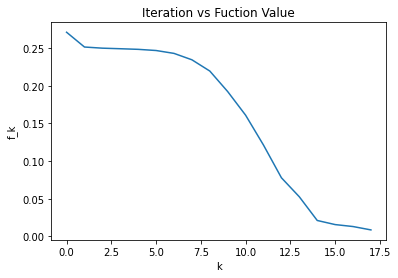
\includegraphics[width=0.7\linewidth]{graficas/sd_f_2}
	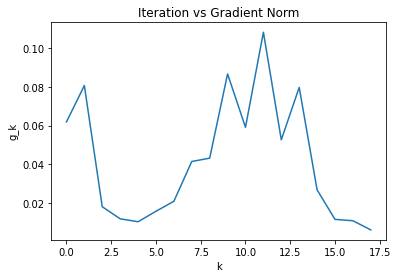
\includegraphics[width=0.7\linewidth]{graficas/sd_g_2}
\end{center}
\subsubsection{BFGS}
\begin{center}
	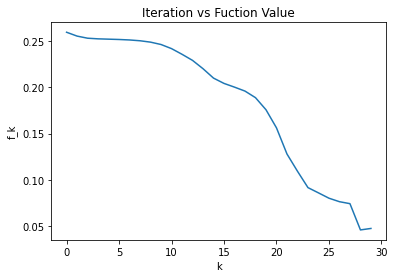
\includegraphics[width=0.7\linewidth]{graficas/bfgs_f_2}
	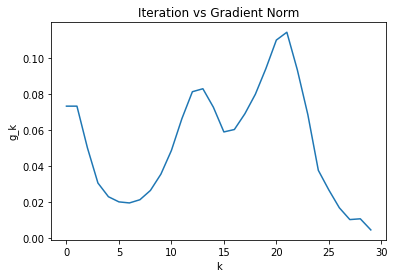
\includegraphics[width=0.7\linewidth]{graficas/bfgs_g_2}
\end{center}
\subsection{$ m = 5 $}
\begin{center}
	\begin{tabular}{cccc}
		\hline
		Algoritmo & tiempo & iteraciones  & error \\
		\hline
		SD   & $ 7345.89 $ segundos & 11 & 0.0037  \\
		BFGS & $ 13974.915 $ segundos  & 21 &0.0099 \\
		\hline
	\end{tabular}
\end{center}
\subsubsection{Descenso Gradiente}
\begin{center}
	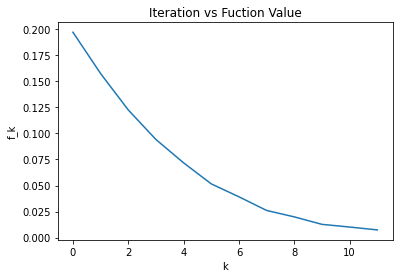
\includegraphics[width=0.7\linewidth]{graficas/sd_f_5}
	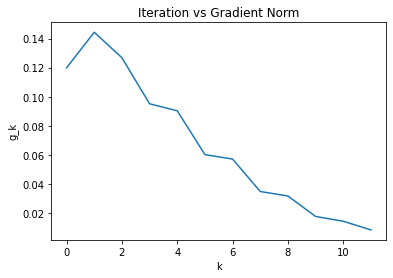
\includegraphics[width=0.7\linewidth]{graficas/sd_g_5}
\end{center}
\subsubsection{BFGS}
\begin{center}
	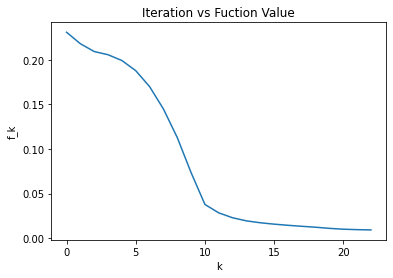
\includegraphics[width=0.7\linewidth]{graficas/bfgs_f_5}
	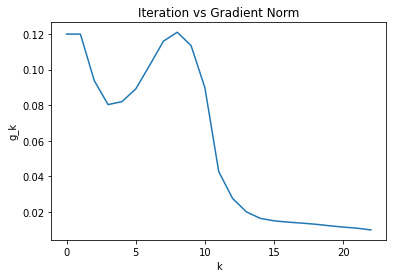
\includegraphics[width=0.7\linewidth]{graficas/bfgs_g_5}
\end{center}


\section{Conclusiones}
	\begin{itemize}
		\item El problema de clasificación binaria de un conjunto de entrenamiento se puede plantear como un problema de optimización. En este caso se usó un conjunto de imágenes de ceros y unos del dataset MNIST. 
		\item En la experimentaicón se observó el costo computacional de no usar directamente el gradiente sino la aproximación de primer orden. Se observó que una evaluación del gradiente tardó entre $ 107 $ y $ 201 $ segundos. Es de esperarse que conforme aumente el valor de $ m $, aumente el tiempo de cálculo. Además, en las gráficas se observó mayor estabilidad a mayor valor de $ m $.
		\item Se observó además que al no obtener directamente la matriz hessiana, el método BFGS es sensible a la inicialización de la matrix $ H $.
		\item El algoritmo BGFS es presenta un buen desempleño y no requiere el cálculo del Hessiano ni de su inversa.
		\item La principal limitación del algoritmo BFGS es en
		problemas donde el número de variable es muy grande (por ejemplo, un millón de variables o más) pues es casi imposible guardar la matriz de tamaño $ n \times n $.
		\item Observemos que el error es pequeño, considerando el número total de imágenes del conjunto de validación. Intuitivamente esto puede ocurrir porque la clasificación es clara para ceros y unos (dado que la forma de escribir estos dígitos es muy diferente). Lo que sugiere probar este algoritmo para clasificar unos y sietes o seis y nueves.
	\end{itemize}
\end{document}